\articlehead{Re-Evalutation Your Sexual Preference}{JM}{2012}

There is a widely-held belief that new furries often re-evaluate their sexual preference after discovering the community.

Stereotypically, a young heterosexual male will begin socializing with furries -- either online or in person -- and will shortly re-evaluate himself as gay (or bi). Our young stereotype may think that furry helped him realize this about himself, and the experience will probably be a very positive one.

Confession time: my name is JM Horse and I am a stereotype.

I first heard about this phenomenon while reading about the community online. The then-popular Furvey, a long furry survey that people would fill in and post to alt.lifestyle.furry on Usenet, had this question (which I have lightly edited for clarity):

\begin{quote}
It is common for many furries to live as a heterosexual, and then through furry to discover their attraction to the same sex -- is this the case with you?
 \end{quote}

This question has been asked since the mid-1990s. But is it true?

I asked Klisoura, who runs the Furry Survey. The chart below shows Klisoura’s data (visualized by Makyo), and it’s remarkable.

\begin{figure}
  \begin{center}
    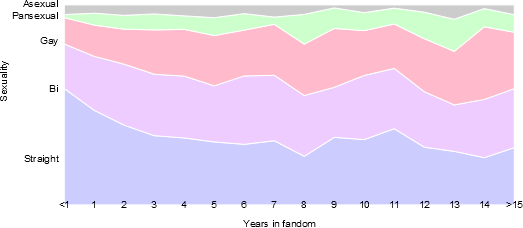
\includegraphics[width=\textwidth]{content/assets/re-evaluating-sexuality--y-o}
  \end{center}
  \caption{Years in the fandom vs. sexual orientation}
\end{figure}

The trend is almost certainly starker than the chart shows. Our first datapoint is based on furries who have been in the community for up to one year. Some of these furries will have already re-evaluated their sexual preference.

It’s safe to conclude that more than half of the heterosexual furries coming into the community will change their sexual preference.

The big question: why is this happening? I have some ideas.

\subsection*{Does furry make you gay?}

No. Furry is no more making people gay than Christian gay-rehabilitation camps are making people straight.

There will, of course, be some heterosexual furries who experiment with gay sex. This happens in every environment: homosexuals often experiment with straight sex when they’re younger; young men brought up in a rural environment often experiment with bestiality. You can’t change, or choose, your sexuality.

\subsection*{Are most people bisexual, and perhaps furry behaviour just a representation of that?}

The idea that most people are bisexual comes from the research of Kinsey and the philosophies of Freud. Both Kinsey and Freud, while very important, have been discredited on this point: Kinsey wildly overestimated the numbers of non-heterosexuals, and Freud believed that homosexuality was a curable mental illness.

Around 2\% of people identify as bisexual, declining with age. Most bisexuals eventually reclassify themselves as straight or gay. However it’s impossible to read much into this as bisexuality is a slippery concept: the ex-bisexuals may be in committed relationships and simply reclassify themselves for clarity.

It’s an interesting and controversial idea, and one that I cannot do justice to here. Suffice to say that there is no evidence for a silent bisexual majority.

The idea, at least in the furry world, can be dismissed by looking at the data. The straight furries who change their sexual preference are much more likely to move from straight to gay, rather than bisexual (or pansexual).

\subsection*{Are furries, to some degree, all zoophiles?}

I suggested in a previous post that furry is a half-step towards zoophilia. However I meant this only from an external perspective -- people unfamiliar with furry may look at all these animal people and jump to a conclusion.

More pertinently, only about 1 in 6 furries identify as zoophiles. That’s a lot but it’s still a small minority.

\subsection*{Is furry a gateway to understanding your true sexuality?}

Possibly.

For most people, it’s not easy growing up gay. It’s assumed that you are straight -- this reference point colours your life as you grow up. Any behaviour that might be homosexual stands out as being different, and nobody wants to be different when they’re an adolescent. You might not meet any openly gay people and if you do, their status as ``gay'' often defines them.

This reference point -- that straight is normal, therefore not-straight is abnormal -- is easy to internalize. A child quickly learns that some thoughts and feelings are acceptable to express out loud, and that some should be hidden. If it feels like you shouldn’t talk about being attracted to the same sex, it can be easy to focus on only those thoughts that reinforce normality. It’s easy to be gay and not know it. It’s easy to be in denial. It’s easy to be gay and homophobic.

Anyone coming out as a gay person has to deal with these two problems -- internalized homophobia and homophobia in society. The first must be overcome to admit to yourself that you are gay.

Perhaps furry is a ‘gateway’ to accepting your true sexuality. For a gay person in denial, it might be easier to enjoy non-human homoerotica without threatening that internalized homophobia.

Furry erotica is stylized. If sex seems a bit smelly or hairy or icky, then furry porn is glossy, neat, and elegant. For a gay furry in denial, it’s a lot easier to fantasize about your furry avatar in a sexual situation compared to imagining yourself in an entanglement with a member of the same sex.

For many furries, consumption of furry erotica is a stepping stone towards becoming a sexually active adult. Furry porn can lead to typesex with an online friend (or stranger), which can lead to flirting and friendly physical contact with furries in real life, which can lead to sex with a likeminded furry. In the best case, this can all occur in an enjoyable, satisfying, low-stress, low-expectation environment.

You don’t have to be a gay furry in denial for this progression to work. There is a preponderance of furries who don’t naturally have a way of expressing their sexuality in the context of normal society. Perhaps the furry community is just a gateway: a way for us to take babysteps to realization of our true sexual identity, whatever that might be.

If this is the case, then furry may simply be a convenient construct. It might be no more than a vehicle that we subconsciously commandeer, taking our conscious mind on a journey to the point where it can accept our sexual needs. To stretch the metaphor, perhaps we can abandon this vehicle once we’ve reached our destination.

(Aside to furries who are currently on the journey: you will get there. You will accept and embrace who you are. You will feel comfortable with yourself and amongst your peers. You will, one day, say out loud ``I am \_\_\_'' and it’ll feel great.)

Perhaps the only reason we stay with the furry group -- once the porn and the community have helped us reach actualization of our true sexuality -- is for our friends, and the fellowship, and the flirtatiousness or sex within the group. Perhaps this explains why 60\% of furries are single; perhaps this explains why furry is so young -- most people move on once they find a long-term relationship.

This is an idea worth exploring in more detail. As a committed furry ``lifestyler'' -- someone who strongly identifies with his furry self and likes to write philosophical articles about the community here on [a][s] -- it’s easy for me to disregard this hypothesis (and, don’t worry, I will in a moment). I’m not an impartial voice: you don’t ask a priest for evidence that god doesn’t exist; you don’t ask a trekkie for an impartial review of William Shatner’s oeuvre.

I think it’s worth entertaining the idea for a moment. If furry were simply a convenient vehicle for each of us to accept and express our true sexuality, we wouldn’t know. The human mind can, and does, keep secrets from itself: a gay person in denial is not aware of something utterly fundamental. We could similarly be non-furries in denial.

Self-deception is a well known phenomenon in cognitive psychology circles, supported by a lot of research and scientific evidence. The basic theory boils down to this: we create a version of the world that is consistent which what we already think. If we see evidence that is contrary to our version of the world, we disregard it in such a way that reinforces our existing belief. This is counterintuitive but true.

So what follows is either my false internal justification for the reality of myself as a furry and the importance of the furry community, or my objective reasoning for such. With that caveat, you may make up your own mind.

\subsection*{My conclusions}

If furry pornography is just a stepping-stone to acceptance of one’s real sexuality, then we would eventually lose interest in furry pornography. We would move on to regular pornography.

It’s not uncommon for pornography to be a gateway. Let’s consider someone with a relatively extreme fetish: a bit of /ah roulette on Fchan has given me castration.

Someone with a fetish for castration is unlikely to leap straight into /ah -- their developing adolescent mind will know that this is not ‘normal’, and so will reject the idea. So our castration-fetishist will find stepping-stones that aren’t too challenging when taken one-at-a-time. Maybe they will start with porn featuring a power imbalance, then maybe knives will come into it, them maybe violence and disfigurement, then maybe slavery and eunuchs, then eventually good-old consensual castration.

Once our castration-lover has accepted their fetish, they will discard the stepping stones and head straight to /ah every time.

Every furry with whom I’ve ever broached the topic is an enthusiastic consumer of furry erotica. For those of us who have accepted our true sexuality, we’re usually consuming regular porn as well. But we’re not discarding the furry stuff.

I’d also argue that all pornography is stylized, not just furry pornography. Regular pornography features people with impossibly little body hair, perfect tans and bleached anuses. For those of you who like body hair: have lots. Like large people? Have really large people. Pornography is always stylized to push our buttons, and it’s evolved this way because that’s what people are demanding. It’s social Darwinism.

More to the point, furry isn’t defined by sex or sexual orientation. Furry is about identity, and that’s what separates it from other fandoms and hobbyist groups. People who identify as a furry usually consider themselves, internally, as a sort of animal-person. And external expression of that internal reality within the furry community can be very rewarding.

I mentioned at the beginning of this article that I am one of those people who re-evaluated their sexual preference after discovering furry. I’d like to share the short version of my story with you.

\begin{quote}
  When I discovered the furry community, I was in a long-term heterosexual relationship with a fantastic person. She and I were great friends and had an active sex life. After a year or so into furry, something new happened: I fell in love with a nominally bisexual furry guy. I broke up with my girlfriend and attempted a new relationship. It didn’t work: the experience made it clear to me that I am gay, and clear to him that he is straight. It was hard on all of us but our friendship trumped the heartbreak. The three of us are still very close friends. A few years ago, I was best man at his wedding.
\end{quote}

My story is unique but typical. I would love to hear your own stories, either in the comments below or elsewhere (jm@furrynet.com).

The furry community is, I think, a great environment for people to get to know themselves. It’s introspective but social; it encourages tolerance and personal growth; it’s trivial and important. I can’t explain why so many furries have unusual sexual and gender identities -- perhaps the heterosexual furries find enough acceptance in the non-furry world, happy enough as Lion King fans, or playing as Khajiit on Skyrim.

I think that there are many people who live as a heterosexual with the subconscious knowledge that they are not being true to themselves. These are people who are not lucky enough to grow up in an environment where sexuality is a preference rather than a potential abnormality, and people who don’t have something like the furry community to help them accept who they really are.

An acquaintance of mine is a palliative care nurse, who provides comfort and dignity to people who are dying. She once told me the biggest regret people have: \textit{``I wish I’d had the courage to live a life true to myself, not the life others expected of me.''}

I feel very lucky to be a stereotype.
